% fig_bridge.tex -- why the self-critical tilt helps: chord subtraction.
% Path realized on the delta = 0.35 testbed, L = 24; coordinates and
% extrema verified in verif_v11/v11_figdata.m.
\begin{tikzpicture}
\begin{axis}[width=8.2cm,height=5.6cm,
  xlabel={context order $k$},ylabel={log-profile},
  xmin=0,xmax=24,ymin=-1.9,ymax=7.4,
  xtick={0,4,8,12,16,20,24},
  legend cell align=left,legend pos=north west,
  legend style={font=\scriptsize,draw=gray!50},
  tick label style={font=\scriptsize},
  label style={font=\scriptsize},
  every axis plot/.append style={thick}]

% the raw fluctuation path D_k (what a fixed beta leaves behind)
\addplot[red!70!black] coordinates {
  (0,0.000)(1,0.601)(2,1.202)(3,1.804)(4,2.405)(5,3.006)(6,3.607)
  (7,4.208)(8,4.809)(9,5.411)(10,4.294)(11,4.895)(12,3.779)(13,4.380)
  (14,4.981)(15,5.582)(16,6.184)(17,5.067)(18,3.951)(19,4.552)
  (20,5.153)(21,4.036)(22,4.638)(23,5.239)(24,5.840)};

% the chord that the self-critical temperature subtracts
\addplot[black,dashed,no marks] coordinates {(0,0)(24,5.840)};

% the resulting bridge B_k, pinned at both ends
\addplot[blue!65!black] coordinates {
  (0,0.000)(1,0.358)(2,0.716)(3,1.074)(4,1.431)(5,1.789)(6,2.147)
  (7,2.505)(8,2.863)(9,3.221)(10,1.861)(11,2.219)(12,0.859)(13,1.217)
  (14,1.575)(15,1.932)(16,2.290)(17,0.930)(18,-0.429)(19,-0.072)
  (20,0.286)(21,-1.074)(22,-0.716)(23,-0.358)(24,0.000)};

\addplot[gray!50,no marks,thin] coordinates {(0,0)(24,0)};

\legend{$D_k$ (fixed $\beta$),chord $\tfrac{k}{L}D_L$,
        $B_k$ (self-critical)}

% mark the two maxima
\addplot[red!70!black,only marks,mark=*,mark size=1.9pt,forget plot]
  coordinates {(16,6.184)};
\addplot[blue!65!black,only marks,mark=*,mark size=1.9pt,forget plot]
  coordinates {(9,3.221)};
\node[font=\scriptsize,red!70!black,anchor=south] at (axis cs:16,6.35)
  {$\max=6.18$};
\node[font=\scriptsize,blue!65!black,anchor=south west]
  at (axis cs:9.3,3.30) {$\max=3.22$};
\node[font=\scriptsize,gray!60!black,anchor=north east]
  at (axis cs:23.6,-0.25) {both ends pinned};
\end{axis}
\end{tikzpicture}
